\chapter{Additional graphs}\label{sec:app:graphs}\thispagestyle{fancy}
%%
%%%%%%%%%% SECTION %%%%%%%%%% {{{1 Edge EC heating replaced by central
\section{Edge EC heating replaced by central}\label{sec:app:graphs:recovery:X3only}
%%
%%%%%%% SUB %%%%%%% {{{2 Profiles
\subsection{Profiles}\label{sec:app:graphs:recovery:X3only:profs}
%%
\begin{AllFigs}{X3onlyNoST}{H}{}{te,ne,lte,lne}{a}{rhosOKplot}{Profiles of the main quantities where we have replaced the edge ECH by central one.}
\end{AllFigs}

\begin{AllFigs}{X3onlyNoST}{H}{}{p_e,ti,itot,ibs,q,shear}{y}{rhosOKplot}{Profiles of the main quantities where we have replaced the edge ECH by central one.}
\end{AllFigs}

\begin{AllFigs}{X3onlyNoST}{H}{}{upl}{y}{rhosOKplot}{Profiles of the main quantities where we have replaced the edge ECH by central one.}
\end{AllFigs}

%% }}}2
%%%%%%% SUB %%%%%%% {{{2 Time traces
\subsection{Time traces}\label{sec:app:graphs:recovery:X3only:traces}
%%
\begin{AllFigs}{X3onlyNoST}{H}{}{te}{a}{resultsplot}{Comparison between experimental profile and only central ECH. The solid blue line is the standard case, the dashed red one is the central ECH one.}
\end{AllFigs}

\begin{AllFigs}{X3onlyNoST}{H}{}{ne,ti,jtot}{y}{resultsplot}{Comparison between experimental profile and only central ECH. The solid blue line is the standard case, the dashed red one is the central ECH one.}
\end{AllFigs}

\begin{AllFigs}{X3onlyNoST}{H}{}{jbs,ibsped,q}{y}{resultsplot}{Comparison between experimental profile and only central ECH. The solid blue line is the standard case, the dashed red one is the central ECH one.}
\end{AllFigs}

\begin{AllFigs}{X3onlyNoST}{H}{}{shear,upl}{y}{resultsplot}{Comparison between experimental profile and only central ECH. The solid blue line is the standard case, the dashed red one is the central ECH one.}
\end{AllFigs}

%% }}}2
%% }}}1
%%%%%%%%%% SECTION %%%%%%%%%% {{{1 Varying $D_n$
\section{Varying $D_n$}\label{sec:app:graphs:recovery:Dn}
%%
%%%%%%% SUB %%%%%%% {{{2 Profiles
\subsection{Profiles}\label{sec:app:graphs:recovery:Dn:profs}
%%
\begin{AllFigs}{Dn10NoST}{H}{}{te,ne,lte,lne,p_e,ti}{a}{rhosOKplot}{Profiles of the main quantities for an inter-ELM with particle diffusivity multiplied by ten.}
\end{AllFigs}

\begin{AllFigs}{Dn10NoST}{H}{}{itot,ibs,q,shear,upl}{y}{rhosOKplot}{Profiles of the main quantities for an inter-ELM with particle diffusivity multiplied by ten.}
\end{AllFigs}

\begin{AllFigs}{Dn05NoST}{H}{}{te,ne,lte,lne,p_e,ti}{a}{rhosOKplot}{Profiles of the main quantities for an inter-ELM with particle diffusivity divided by two.}
\end{AllFigs}

\begin{AllFigs}{Dn05NoST}{H}{}{itot,ibs,q,shear,upl}{y}{rhosOKplot}{Profiles of the main quantities for an inter-ELM with particle diffusivity divided by two.}
\end{AllFigs}

\begin{AllFigs}{Dn01NoST}{H}{}{te,lte,lne,p_e,ti,itot}{a}{rhosOKplot}{Profiles of the main quantities for an inter-ELM with particle diffusivity divided by ten.}
\end{AllFigs}

\begin{AllFigs}{Dn01NoST}{H}{}{ibs,q,shear,upl}{y}{rhosOKplot}{Profiles of the main quantities for an inter-ELM with particle diffusivity divided by ten.}
\end{AllFigs}

%% }}}2
%%%%%%% SUB %%%%%%% {{{2 Time traces
\subsection{Time traces}\label{sec:app:graphs:recovery:Dn:traces}
%%
\begin{AllFigs}{DnNoST}{H}{}{q}{a}{resultsplot}{Comparison between different values for Dn. The solid blue line is the reference case, the dashed red one is the ``Dn10'' case, the dash-dotted dark green is ``Dn05'' and the dotted black is ``Dn01''.}
\end{AllFigs}
%% }}}2
%%%%%%% SUB %%%%%%% {{{2 MHD diagrams
\subsection{MHD diagrams}\label{sec:app:graphs:recovery:Dn:jalpha}
%%
\begin{figure}[H]
\begin{center}
\includegraphics[height=8cm,width=12cm]{../matlab/pics/40080_0.8_jalpha_Dn10NoST.eps}
\vspace{-0.5cm}
\end{center}
\caption{\footnotesize $j - \alpha$ diagram for the ``Dn10'' ELM cycle. Dotted lines are during the ELM crash $0 \le t <0.1$, dash-dotted is for $0.1 \le t < 0.5$, solid lines are $0.5 \le t < 1$ and dashed lines are from 1 to the next ELM (20) with the time in $ms$. $\rho_V = 0.75$ is the top of the density pedestal, $\rho_V = 0.79$ is where this diagram is the largest, $\rho_V = 0.81$ is the top of the temperature pedestal and $\rho_V = 0.86$ is the maximum of the pressure gradient.\label{fig:results:ELM:Dn10:jalpha}}
\vspace{-0.5cm}
\end{figure}
%%
\begin{figure}[H]
\begin{center}
\includegraphics[height=8cm,width=12cm]{../matlab/pics/40080_0.8_jalpha_Dn05NoST.eps}
\vspace{-0.5cm}
\end{center}
\caption{\footnotesize $j - \alpha$ diagram for the ``Dn05'' ELM cycle. Dotted lines are during the ELM crash $0 \le t <0.1$, dash-dotted is for $0.1 \le t < 0.5$, solid lines are $0.5 \le t < 1$ and dashed lines are from 1 to the next ELM (20) with the time in $ms$. $\rho_V = 0.75$ is the top of the density pedestal, $\rho_V = 0.79$ is where this diagram is the largest, $\rho_V = 0.81$ is the top of the temperature pedestal and $\rho_V = 0.86$ is the maximum of the pressure gradient.\label{fig:results:ELM:Dn05:jalpha}}
\vspace{-0.5cm}
\end{figure}
%% }}}2
%% }}}1
%%%%%%%%%% SECTION %%%%%%%%%% {{{1 First vs non-first
\section{First vs non-first}\label{sec:app:graphs:recovery:first}
%%
%%%%%%% SUB %%%%%%% {{{2 Reference case
\subsection{Reference case}\label{sec:app:graphs:recovery:first:std}
%%
%%%% SUB-SUB %%%% {{{3 Profiles
\subsubsection{Profiles}\label{sec:app:graphs:recovery:first:std:profs}
%%
\begin{AllFigs}{stdNoSTfirst}{H}{}{te,ne,lte,lne,p_e,ti}{a}{rhosOKplot}{Profiles of the main quantities for an inter-ELM in the reference case for the first ELM.}
\end{AllFigs}

\begin{AllFigs}{stdNoSTfirst}{H}{}{itot,ibs,q,shear,upl}{y}{rhosOKplot}{Profiles of the main quantities for an inter-ELM in the reference case for the first ELM.}
\end{AllFigs}
%% }}}3
%%%% SUB-SUB %%%% {{{3 Time traces
\subsubsection{Time traces}\label{sec:app:graphs:recovery:first:std:traces}
%%
\begin{AllFigs}{stdNoSTfirst}{H}{}{te,p_e,ti}{a}{resultsplot}{Comparison between first and non-first ELM. The solid blue line is the non-first from the standard case while the dashed red one is the first.}
\end{AllFigs}

\begin{AllFigs}{stdNoSTfirst}{H}{}{jtot,jbs,ibsped}{y}{resultsplot}{Comparison between first and non-first ELM. The solid blue line is the non-first from the standard case while the dashed red one is the first.}
\end{AllFigs}

\begin{AllFigs}{stdNoSTfirst}{H}{}{q,shear,upl}{y}{resultsplot}{Comparison between first and non-first ELM. The solid blue line is the non-first from the standard case while the dashed red one is the first.}
\end{AllFigs}
%% }}}3
%% }}}2
%%%%%%% SUB %%%%%%% {{{2 Particle diffusivity multiplied by ten
\subsection{Particle diffusivity multiplied by ten}\label{sec:app:graphs:recovery:first:Dn10}
%%
%%%% SUB-SUB %%%% {{{3 Profiles
\subsubsection{Profiles}\label{sec:app:graphs:recovery:first:Dn10:profiles}
%%
\begin{AllFigs}{Dn10NoSTfirst}{H}{}{te,ne,lte,lne,p_e,ti}{a}{rhosOKplot}{Profiles of the main quantities for an inter-ELM for the case ``Dn10'' for the first ELM.}
\end{AllFigs}

\begin{AllFigs}{Dn10NoSTfirst}{H}{}{itot,ibs,q,shear,upl}{y}{rhosOKplot}{Profiles of the main quantities for an inter-ELM for the case ``Dn10'' for the first ELM.}
\end{AllFigs}
%% }}}3
%%%% SUB-SUB %%%% {{{3 Time traces
\subsubsection{Time traces}\label{sec:app:graphs:recovery:first:Dn10:traces}
%%
\begin{AllFigs}{Dn10NoSTfirst}{H}{}{te,ne,p_e}{a}{resultsplot}{Comparison between first and non-first ELM. The solid blue line is the non-first from case ``Dn10'' while the dashed red one is the first.}
\end{AllFigs}

\begin{AllFigs}{Dn10NoSTfirst}{H}{}{ti,jtot,jbs}{y}{resultsplot}{Comparison between first and non-first ELM. The solid blue line is the non-first from case ``Dn10'' while the dashed red one is the first.}
\end{AllFigs}

\begin{AllFigs}{Dn10NoSTfirst}{H}{}{ibsped,q,shear}{y}{resultsplot}{Comparison between first and non-first ELM. The solid blue line is the non-first from case ``Dn10'' while the dashed red one is the first.}
\end{AllFigs}

\begin{AllFigs}{Dn10NoSTfirst}{H}{}{upl}{y}{resultsplot}{Comparison between first and non-first ELM. The solid blue line is the non-first from case ``Dn10'' while the dashed red one is the first.}
\end{AllFigs}
%% }}}3
%%%% SUB-SUB %%%% {{{3 MHD diagram
\subsubsection{MHD diagram}\label{sec:app:graphs:recovery:first:Dn10:jalpha}
%%
\begin{figure}[H]
\begin{center}
\includegraphics[height=8cm,width=12cm]{../matlab/pics/40080_0.8_jalpha_Dn10NoSTfirst.eps}
\vspace{-0.5cm}
\end{center}
\caption{\footnotesize $j - \alpha$ diagram for the first ELM cycle of the ``Dn10'' case. Dotted lines are during the ELM crash $0 \le t <0.1$, dash-dotted is for $0.1 \le t < 0.5$, solid lines are $0.5 \le t < 1$ and dashed lines are from 1 to the next ELM (20) with the time in $ms$. $\rho_V = 0.75$ is the top of the density pedestal, $\rho_V = 0.79$ is where this diagram is the largest, $\rho_V = 0.81$ is the top of the temperature pedestal and $\rho_V = 0.86$ is the maximum of the pressure gradient.\label{fig:results:ELM:Dn10first:jalpha}}
\vspace{-0.5cm}
\end{figure}
%% }}}3
%% }}}2
%%%%%%% SUB %%%%%%% {{{2 Particle diffusivity divided by two
\subsection{Particle diffusivity divided by two}\label{sec:app:graphs:recovery:first:Dn05}
%%
%%%% SUB-SUB %%%% {{{3 Profiles
\subsubsection{Profiles}\label{sec:app:graphs:recovery:first:Dn05:profiles}
%%
\begin{AllFigs}{Dn05NoSTfirst}{H}{}{te,ne,lte,lne,p_e,ti}{a}{rhosOKplot}{Profiles of the main quantities for an inter-ELM for the case ``Dn05'' for the first ELM.}
\end{AllFigs}

\begin{AllFigs}{Dn05NoSTfirst}{H}{}{itot,ibs,q,shear,upl}{y}{rhosOKplot}{Profiles of the main quantities for an inter-ELM for the case ``Dn05'' for the first ELM.}
\end{AllFigs}
%% }}}3
%%%% SUB-SUB %%%% {{{3 Time traces
\subsubsection{Time traces}\label{sec:app:graphs:recovery:first:Dn05:traces}
%%
\begin{AllFigs}{Dn05NoSTfirst}{H}{}{te,ne,p_e}{a}{resultsplot}{Comparison between first and non-first ELM. The solid blue line is the non-first from the half-diffusivity case while the dashed red one is the first.}
\end{AllFigs}

\begin{AllFigs}{Dn05NoSTfirst}{H}{}{ti,jtot,jbs}{y}{resultsplot}{Comparison between first and non-first ELM. The solid blue line is the non-first from the half-diffusivity case while the dashed red one is the first.}
\end{AllFigs}
\begin{AllFigs}{Dn05NoSTfirst}{H}{}{ibsped,q,shear}{y}{resultsplot}{Comparison between first and non-first ELM. The solid blue line is the non-first from the half-diffusivity case while the dashed red one is the first.}
\end{AllFigs}
\begin{AllFigs}{Dn05NoSTfirst}{H}{}{upl}{y}{resultsplot}{Comparison between first and non-first ELM. The solid blue line is the non-first from the half-diffusivity case while the dashed red one is the first.}
\end{AllFigs}
%% }}}3
%%%% SUB-SUB %%%% {{{3 MHD diagram
\subsubsection{MHD diagram}\label{sec:app:graphs:recovery:first:Dn05:jalpha}
%%
\begin{figure}[H]
\begin{center}
\includegraphics[height=8cm,width=12cm]{../matlab/pics/40080_0.8_jalpha_Dn05NoSTfirst.eps}
\vspace{-0.5cm}
\end{center}
\caption{\footnotesize $j - \alpha$ diagram for the first ELM cycle of the ``Dn05'' case. Dotted lines are during the ELM crash $0 \le t <0.1$, dash-dotted is for $0.1 \le t < 0.5$, solid lines are $0.5 \le t < 1$ and dashed lines are from 1 to the next ELM (20) with the time in $ms$. $\rho_V = 0.75$ is the top of the density pedestal, $\rho_V = 0.79$ is where this diagram is the largest, $\rho_V = 0.81$ is the top of the temperature pedestal and $\rho_V = 0.86$ is the maximum of the pressure gradient.\label{fig:results:ELM:Dn05first:jalpha}}
\vspace{-0.5cm}
\end{figure}
%% }}}3
%% }}}2
%%%%%%% SUB %%%%%%% {{{2 Particle diffusivity divided by ten
\subsection{Particle diffusivity divided by ten}\label{sec:app:graphs:recovery:first:Dn01}
%%
%%%% SUB-SUB %%%% {{{3 Profiles
\subsubsection{Profiles}\label{sec:app:graphs:recovery:first:Dn01:profiles}
%%
\begin{AllFigs}{Dn01NoSTfirst}{H}{}{te,ne,lte,lne,p_e,ti}{a}{rhosOKplot}{Profiles of the main quantities for an inter-ELM for the case ``Dn01'' for the first ELM.}
\end{AllFigs}

\begin{AllFigs}{Dn01NoSTfirst}{H}{}{itot,ibs,q,shear,upl}{y}{rhosOKplot}{Profiles of the main quantities for an inter-ELM for the case ``Dn01'' for the first ELM.}
\end{AllFigs}
%% }}}3
%%%% SUB-SUB %%%% {{{3 Time traces
\subsubsection{Time traces}\label{sec:app:graphs:recovery:first:Dn01:traces}
%%
\begin{AllFigs}{Dn01NoSTfirst}{H}{}{ibsped}{a}{resultsplot}{Comparison between first and non-first ELM. The solid blue line is the non-first from the ``Dn01'' case while the dashed red one is the first.}
\end{AllFigs}
%% }}}3
%%%% SUB-SUB %%%% {{{3 MHD diagram
\subsubsection{MHD diagram}\label{sec:app:graphs:recovery:first:Dn01:jalpha}
%%
\begin{figure}[H]
\begin{center}
\includegraphics[height=8cm,width=12cm]{../matlab/pics/40080_0.8_jalpha_Dn01NoSTfirst.eps}
\vspace{-0.5cm}
\end{center}
\caption{\footnotesize $j - \alpha$ diagram for the first ELM cycle of the ``Dn01'' case. Dotted lines are during the ELM crash $0 \le t <0.1$, dash-dotted is for $0.1 \le t < 0.5$, solid lines are $0.5 \le t < 1$ and dashed lines are from 1 to the next ELM (20) with the time in $ms$. $\rho_V = 0.75$ is the top of the density pedestal, $\rho_V = 0.79$ is where this diagram is the largest, $\rho_V = 0.81$ is the top of the temperature pedestal and $\rho_V = 0.86$ is the maximum of the pressure gradient.\label{fig:results:ELM:Dn01first:jalpha}}
\vspace{-0.5cm}
\end{figure}
%% }}}3
%% }}}2
%% }}}1
%%%%%%%%%% SECTION %%%%%%%%%% {{{1 Comparing the change in $D_n$ to that in the ELM period
\section{Comparing the change in $D_n$ to that in the ELM period}\label{sec:app:graphs:recovery:delta}
%%
%%%%%%% SUB %%%%%%% {{{2 Profiles
\subsection{Profiles}\label{sec:app:graphs:recovery:delta:profiles}
%%
\begin{AllFigs}{delta05NoST}{H}{}{te,ne,lte,lne,p_e,ti}{a}{rhosOKplot}{Profiles of the main quantities for an inter-ELM for when dividing the ELM period by two.}
\end{AllFigs}

\begin{AllFigs}{delta05NoST}{H}{}{itot,ibs,q,shear,upl}{y}{rhosOKplot}{Profiles of the main quantities for an inter-ELM for when dividing the ELM period by two.}
\end{AllFigs}
%% }}}2
%%%%%%% SUB %%%%%%% {{{2 Time traces
\subsection{Time traces}\label{sec:app:graphs:recovery:delta:traces}
%%
\begin{AllFigs}{DnVSdeltaNoST}{H}{}{te,p_e,ti}{a}{resultsplot}{Comparison between changing $D_n$ and the ELM period.}
\end{AllFigs}

\begin{AllFigs}{DnVSdeltaNoST}{H}{}{jtot,jbs,ibsped}{y}{resultsplot}{Comparison between changing $D_n$ and the ELM period.}
\end{AllFigs}

\begin{AllFigs}{DnVSdeltaNoST}{H}{}{q,shear,upl}{y}{resultsplot}{Comparison between changing $D_n$ and the ELM period.}
\end{AllFigs}
%% }}}2
%%%%%%% SUB %%%%%%% {{{2 MHD diagram
\subsection{MHD diagram}\label{sec:app:graphs:recovery:delta:jalpha}
%%
\begin{figure}[H]
\begin{center}
\includegraphics[height=8cm,width=12cm]{../matlab/pics/40080_0.8_jalpha_delta05NoST.eps}
\vspace{-0.5cm}
\end{center}
\caption{\footnotesize $j - \alpha$ diagram for the ELM cycle with half the period. Dotted lines are during the ELM crash $0 \le t <0.1$, dash-dotted is for $0.1 \le t < 0.5$, solid lines are $0.5 \le t < 1$ and dashed lines are from 1 to the next ELM (10) with the time in $ms$. $\rho_V = 0.75$ is the top of the density pedestal, $\rho_V = 0.79$ is where this diagram is the largest, $\rho_V = 0.81$ is the top of the temperature pedestal and $\rho_V = 0.86$ is the maximum of the pressure gradient.\label{fig:results:ELM:delta05:jalpha}}
\vspace{-0.5cm}
\end{figure}
%% }}}2
%% }}}1
%%%%%%%%%% SECTION %%%%%%%%%% {{{1 Doubling the ELM interaction region
\section{Doubling the ELM interaction region}\label{sec:app:graphs:recovery:rhoELM}
%%
\begin{AllFigs}{width2NoST}{H}{}{lte,lne,p_e,ti,itot,ibs}{a}{rhosOKplot}{Profiles of the main quantities for the case where we double the ELM range.}
\end{AllFigs}

\begin{AllFigs}{width2NoST}{H}{}{q,shear,upl}{y}{rhosOKplot}{Profiles of the main quantities for the case where we double the ELM range.}
\end{AllFigs}
%% }}}1
